\section{Introduction}

\begin{figure*}[ht]
    \centering
	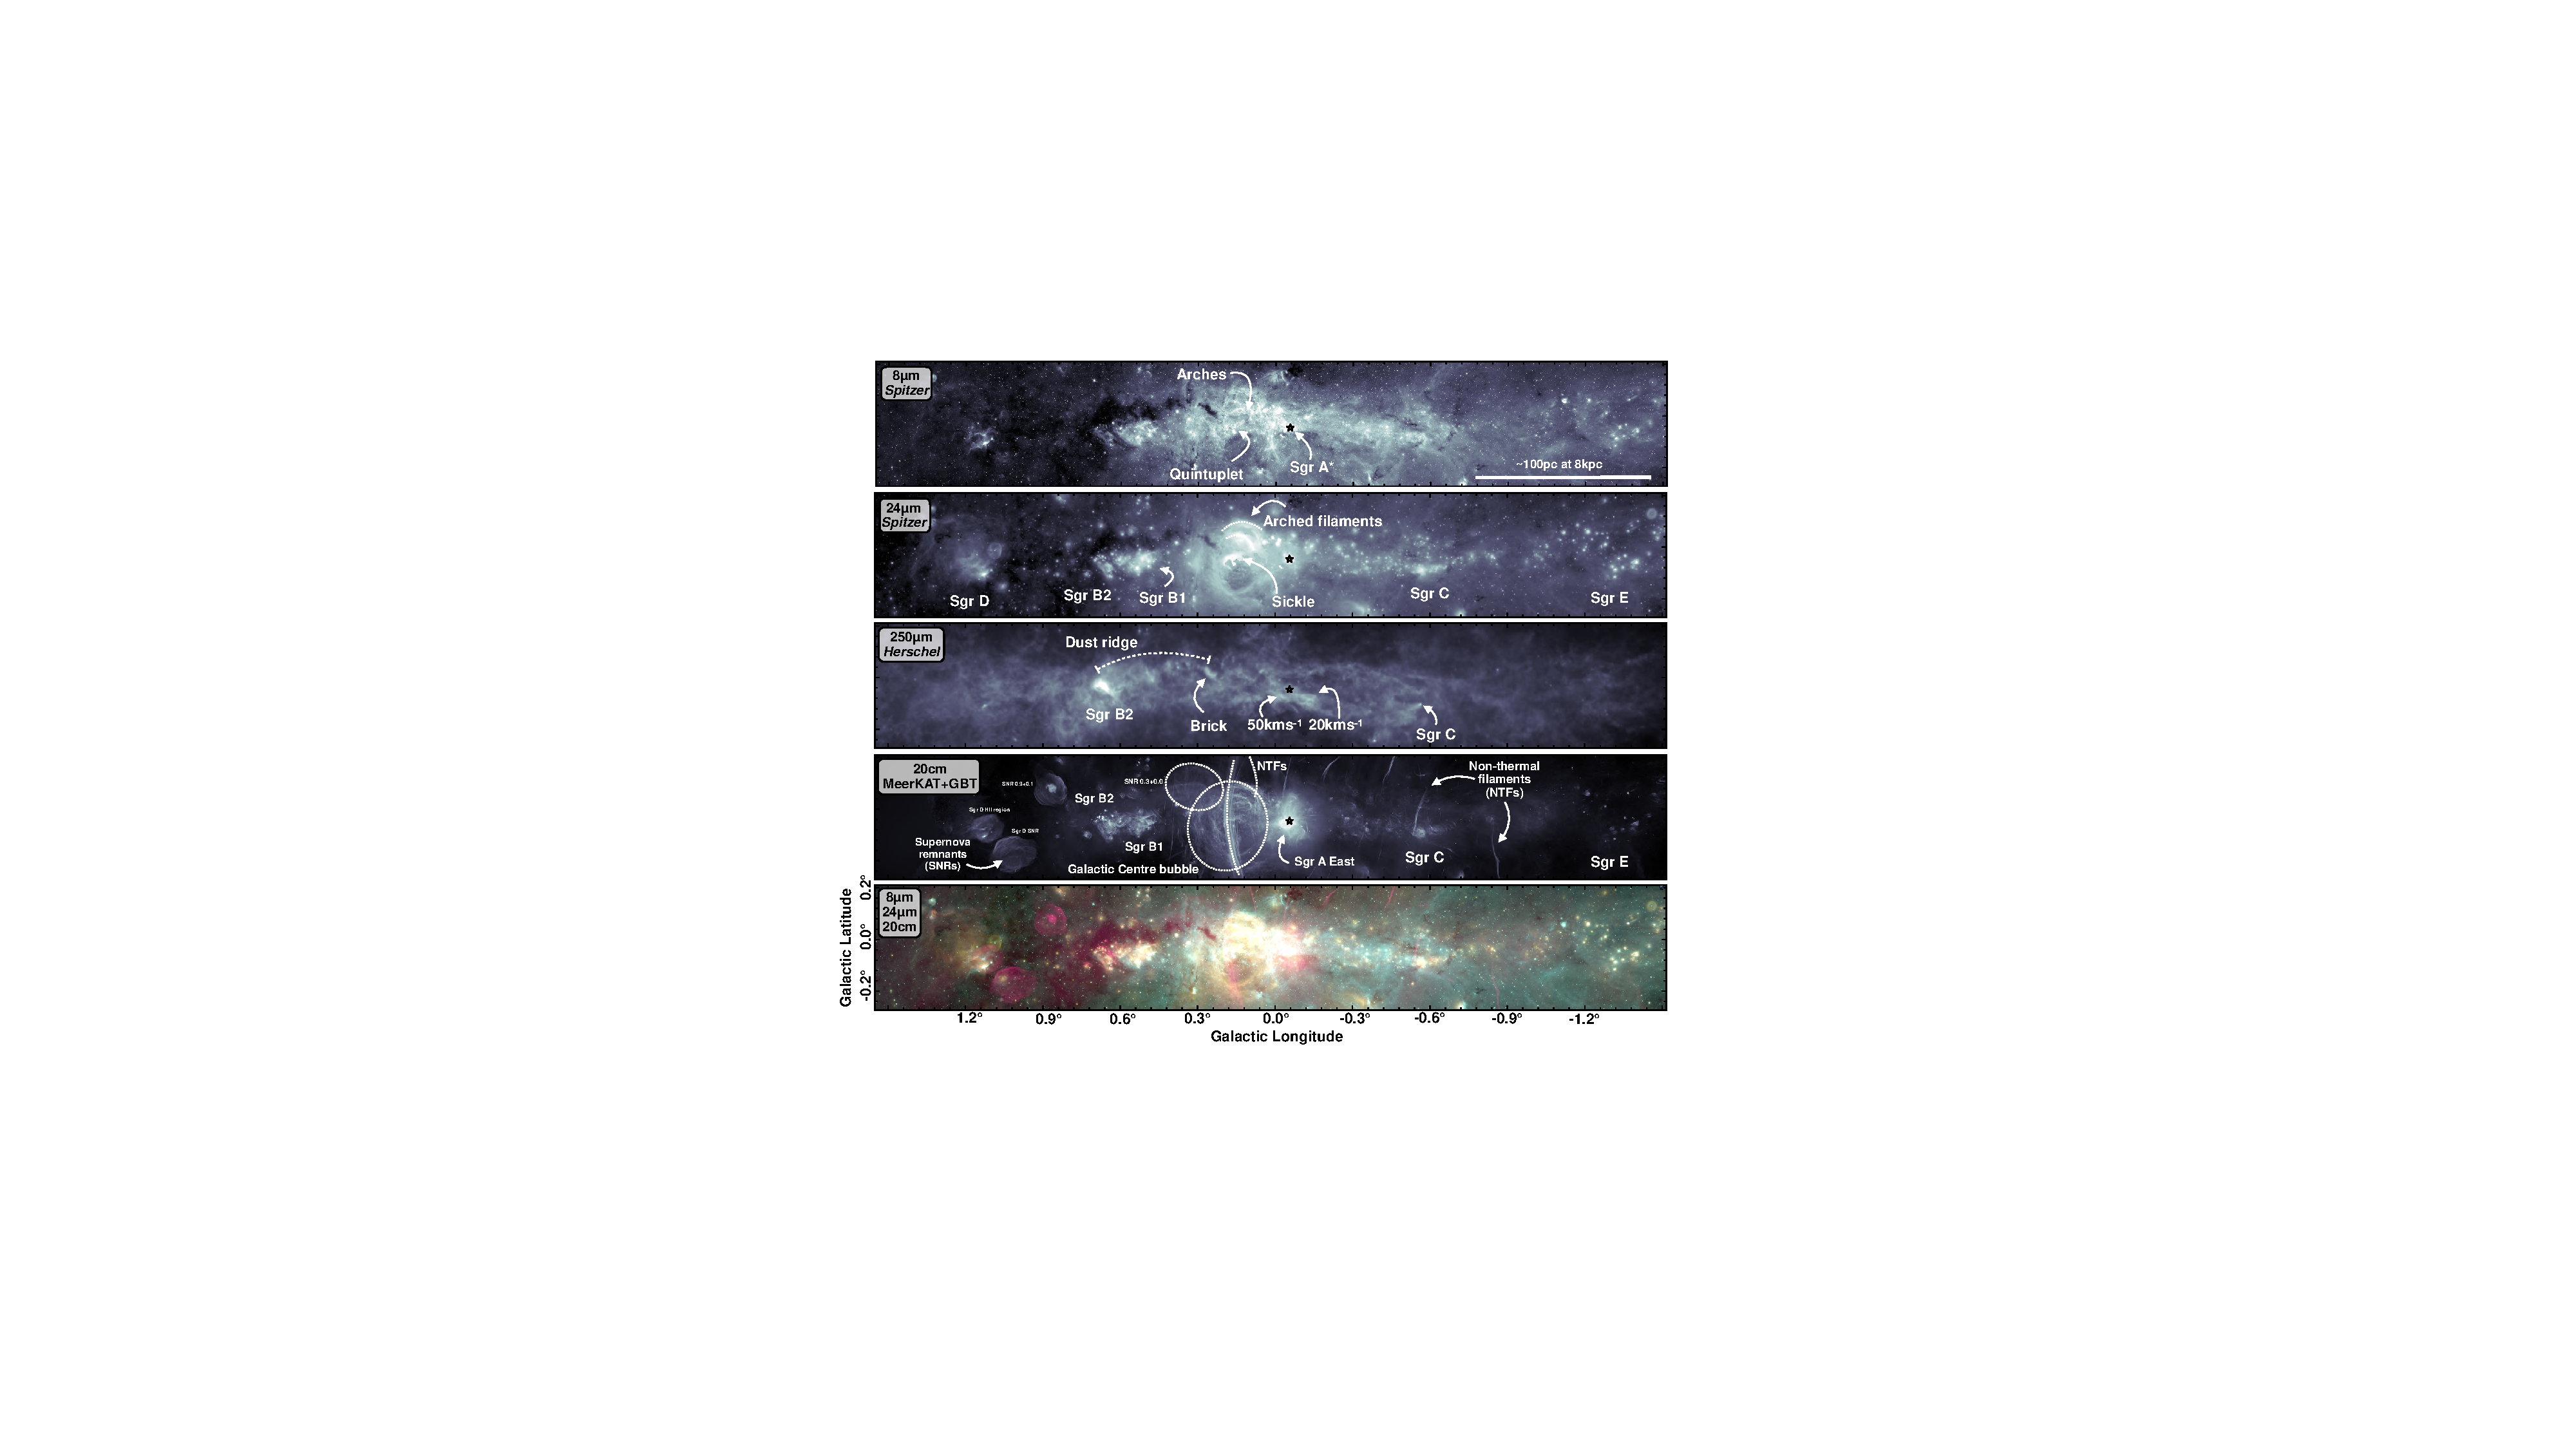
\includegraphics[trim=0 0cm 0 0cm, clip, width=0.9\textwidth]{./figs/rgb_v2_compressed.pdf}
    \caption{A multi-wavelength view of the CMZ. From top to bottom: 8\micron\ emission from the {\em Spitzer} GLIMPSE survey \citep{Churchwell2009}, 24\micron\ emission from the {\em Spitzer} MIPSGAL survey \citep{Carey2009}, 250\micron\ emission from the {\em Herschel} Hi-GAL survey \citep{Molinari2010}, and 20\,cm emission observed by MeerKAT \citep{Heywood2019, Heywood2022} and the Green Bank Telescope (GBT; \citealp{Law2008}). The bottom panel is a three-colour composite of the 8\micron\ (green), 24\micron\ (yellow) and 20\,cm (red) emission. Overlaid are labels highlighting several features of interest. 
    }
    \label{fig:rgb_main}
\end{figure*}

Understanding the formation process of stars and planets is one of the most prominent unsolved problems in contemporary astrophysics.
In particular, establishing what role, if any, environment plays in controlling important quantities, such as the rate and efficiency of star formation, as well as the properties of formed stars, such as their mass distribution at birth and how they cluster together in space and time, has profound implications for our understanding of how galaxies evolve across cosmic time. 

Much of our detailed knowledge of star and planet formation comes from molecular clouds located within $\sim500$\,pc of the Sun. Because these clouds are nearby, their embedded star formation can be studied in exquisite detail, from the cloud-scale down to the scales of individual protoplanetary discs. As a result, molecular clouds in the Solar neighbourhood have been instrumental in shaping our understanding of the structure of the cold interstellar medium (ISM) and of the process of (low-mass) star formation \citep{Ward-Thompson2007,Andre2014, Padoan2014}. As already documented throughout the Protostars \& Planets series, under the typical conditions found in the Solar neighbourhood and, more generally, the disc of the Milky Way, stars typically form in filaments \citep[][see also Pineda et al. and Hacar et al. this volume]{Andre2014}, and the mass distribution of their embedded core populations (i.e. the core mass function, CMF) and the emergent stellar initial mass function \citep[IMF;][]{Offner2014} show remarkably little variation. However, the narrow range of ISM conditions found in nearby clouds is a limiting factor in the development of a general theory for star formation. 

In the context of Galactic star formation, the Central Molecular Zone (i.e. the region within a Galactocentric radius of $R\simeq300$\,pc, hereafter, the CMZ), is an environment like no other. The CMZ hosts the nearest supermassive black hole, some of the closest and most massive young star clusters, the largest number of supernovae per unit volume, complex dynamics driven by the non-axisymmetric gravitational field of the Galactic bar, and it is the largest concentration of dense molecular gas in the Galaxy (see Fig.~\ref{fig:rgb_main}).
The ISM conditions at the centre of the Galaxy are extreme compared to the Solar neighbourhood. Turbulent motions, magnetic field strengths, gas densities, pressures, and temperatures are orders of magnitude greater than those measured locally. 
Many of these properties are more similar to those found at earlier epochs in the Universe \citep{Kruijssen2013}. 
Beyond the Milky Way, the centres of galaxies play an important role in galaxy evolution. They can contribute anywhere from $\sim$a few \% to $>80$\% of the overall star formation of their host galaxy \citep{Kormendy2004}, and the large-scale outflows launched by either central starbursts or active galactic nuclei (AGN) can drive the evolution of their host via the inside-out cessation (or ``quenching'') of star formation \citep{Veilleux2020}. 

The centre of the Milky Way is currently the only galactic nucleus in which it is possible to resolve the multi-scale physics of star formation down to the scales of protoplanetary discs. 
In a Galactic context, the CMZ is a unique region where current theories of star and planet formation can be bench-marked and tested.
In an extragalactic context, the CMZ is a \emph{rosetta stone}: a template to understand extragalactic nuclei and a potential window into earlier epochs in the Universe. Our review focuses on the recent advances in the field of star formation in the CMZ. It is organised as follows. In \S\ref{sec:IG} we describe the landscape of the inner Galaxy and the dynamical origin of the CMZ. In \S\ref{sec:global}, we review the global picture and evolution of CMZ star formation. \S\ref{sec:macroevolution} covers the macro-evolution of the CMZ, and the balance between inflow, outflow, and the central gas reservoir. In \S\ref{sec:cloudtodisc} and \S\ref{sec:environmentofstarformation}, we zoom in, and review the recent body of work dedicated to studying the population of extreme molecular clouds, and the process of star formation embedded within them. Finally, in \S\ref{sec:summary}, we discuss critical open questions and highlight important avenues for future studies.


